\documentclass{article}
\usepackage{amsmath}
\usepackage{bm}
\usepackage{float}
\usepackage{graphicx}
\usepackage[utf8]{inputenc}
\graphicspath{{./images/}}

\title{University Physics with Modern Physics Mechanics Notes}
\author{Chris Doble}
\date{October 2022}

\begin{document}

\maketitle

\tableofcontents

\section{Units, Physical Quantities, and Vectors}

\setcounter{subsection}{4}
\subsection{Uncertainty and Significant Figures}

\begin{itemize}
  \item If the uncertainty of a number isn't explicitly stated it can be indicated by the number of meaningful digits which is the number of digits excluding leading zeros, e.g. $0.1$ and $1$ have one, $1.0$ has two, and $1.00$ has three

  \item It is assumed that the value has an uncertainty $\pm$ one unit of the least significant digit, e.g. $1$ is $\pm1$, $0.1$ and $1.0$ are $\pm0.1$, and $1.00$ is $\pm0.01$

  \item When you multiply or divide numbers with uncertainties the result can have no more significant figures than the input with the fewest significant figures, e.g. $3.1416 \times 2.34 \times 0.58 = 4.3$

  \item When you add or subtract numbers with uncertainties the number of significant figures in the result is determined by the term with the largest uncertainty, e.g. $123.62 + 8.9 = 132.5$

  \item When reducing the number of significant figures in a result round rather than truncate, e.g. $1.688102894$ to three significant figures is $1.69$ not $1.68$

  \item For the most accurate results, preserve extra significant figures throughout a calculation and only round the result
\end{itemize}

\section{Motion Along a Straight Line}

\setcounter{subsection}{3}
\subsection{Motion with Constant Acceleration}

\begin{itemize}
  \item $v_x=v_{0x}+a_xt$

  \item $x=x_0+v_{0x}t+\frac{1}{2}a_xt^2$

  \item $v_x^2=v_{0x}^2+2a_x\left(x-x_0\right)$

  \item $x-x_0=\frac{1}{2}\left(v_{0x}+v_x\right)t$
\end{itemize}

\section{Motion in Two or Three Dimensions}

\subsection{Position and Velocity Vectors}

\begin{itemize}
  \item $\mathbf{r}=x\hat{\mathbf{i}}+y\hat{\mathbf{j}}+z\hat{\mathbf{k}}$

  \item $\mathbf{v}_{av}=\frac{\Delta\mathbf{r}}{\Delta t}$

  \item $\mathbf{v}=\frac{d\mathbf{r}}{dt}$
\end{itemize}

\subsection{The Acceleration Vector}

\begin{itemize}
  \item $\mathbf{a}_{av}=\frac{\Delta\mathbf{v}}{\Delta t}$

  \item $\mathbf{a}=\frac{d\mathbf{v}}{dt}$

  \item $\mathbf{a}$ can be decomposed into $\mathbf{a}_\parallel$, the component parallel to $\mathbf{v}$ which affects speed, and $\mathbf{a}_\perp$, the component perpendicular to $\mathbf{v}$ which affects direction
\end{itemize}

\setcounter{subsection}{3}
\subsection{Uniform Circular Motion}

\begin{itemize}
  \item $a_{rad}=\frac{v^2}{R}$

  \item $T=\frac{2\pi R}{v}$

  \item $a_{rad}=\frac{4\pi^2R}{T^2}$

  \item Because the acceleration in uniform circular motion is always directed towards the centre of the circle, it is sometimes called \textbf{centripetal acceleration} meaning "seeking the centre"

  \item $a_{tan}=\frac{dv}{dt}$
\end{itemize}

\subsection{Relative Velocity}

\begin{itemize}
  \item An observer equipped with a meter stick and a stopwatch forms a \textbf{frame of reference} — a coordinate system plus a time scale

  \item The position of a point or frame of reference A relative to a frame of reference B is given by $\mathbf{r}_{A/B}$ and its velocity is given by $\mathbf{v}_{A/B-x}$

  \item $\mathbf{r}_{P/A}=\mathbf{r}_{P/B}+\mathbf{r}_{B/A}$

  \item $\mathbf{v}_{P/A}=\mathbf{v}_{P/B}+\mathbf{v}_{B/A}$
\end{itemize}

\section{Newton's Laws of Motion}

\subsection{Force and Interactions}

\begin{itemize}
  \item The principle of \textbf{superposition of forces} states that any number of forces applied at a point on an object have the same effect as a single force equal to the vector sum of the forces

  \item The net force acting on an object is $\mathbf{R}=\Sigma\mathbf{F}=\mathbf{F}_1+\mathbf{F}_2+\cdots$
\end{itemize}

\subsection{Newton's First Law}

\begin{itemize}
  \item \textbf{Newton's first law of motion} states: An object acted on by no net external force has constant velocity (which may be zero) and zero acceleration

  \item Newton's first law only applies in \textbf{inertial frames of reference}, i.e. frames of reference that aren't undergoing acceleration
\end{itemize}

\subsection{Newton's Second Law}

\begin{itemize}
  \item \textbf{Newton's second law of motion} states: If a net external force acts on an object, the object accelerates. The direction of acceleration is the same as the direction of the net external force. The mass of the object times the acceleration vector of the object equals the net external force vector

  \item $\mathbf{F}=\frac{d\mathbf{p}}{dt}=\frac{d\left(m\mathbf{v}\right)}{dt}=m\frac{d\mathbf{v}}{dt}=m\mathbf{a}$

  \item Newton's second law only applies in \textbf{inertial frames of reference}, i.e. frames of reference that aren't undergoing acceleration
\end{itemize}

\subsection{Newton's Third Law}

\begin{itemize}
  \item \textbf{Newton's third law of motion} states: If object A exerts a force on object B (an "action"), then object B exerts a force on object A (a "reaction"). These two forces have the same magnitude but are opposite in direction. These two forces act on different objects.
\end{itemize}

\section{Applying Newton's Laws}

\setcounter{subsection}{2}
\subsection{Friction Forces}

\begin{itemize}
  \item Friction forces always oppose the direction of motion

  \item The friction that acts when an object slides over a surface is called \textbf{kinetic friction} and is proportional to the normal force \[f_k=\mu_k n\] where $f_k$ is the magnitude of the kinetic friction force, $\mu_k$ is the \textbf{coefficient of kinetic friction}, and $n$ is the magnitude of the normal force

  \item The friction that acts when an object isn't yet moving is called \textbf{static friction} and is proportional to the normal force \[f_s\le\left(f_s\right)_\textrm{max}=\mu_s n\] where $f_s$ is the magnitude of the static friction force, $\left(f_s\right)_\textrm{max}$ is the maximum magnitude of the static friction force, $\mu_s$ is the \textbf{coefficient of static friction}, and $n$ is the magnitude of the normal force

  \item \textbf{Rolling resistance} is the force resisting motion when a body such as a ball, tire, or wheel rolls on a surface. It includes factors such as deformation of the surface, friction between bearings, etc. \[f_r=\mu_r n\] where $f_r$ is the magnitude of the rolling resistance, $\mu_r$ is the \textbf{coefficient of rolling friction}, and $n$ is the magnitude of the normal force

  \item The force that a fluid (a gas or liquid) exerts on an object moving through it is known as \textbf{fluid resistance}. It opposes the direction of motion and, for small objects moving at low speeds, is proportional to the object's velocity \[f=kv\] where $f$ is the magnitude of the fluid resistance, $k$ is a proportionality constant that depends on the shape and size of the object and the properties of the fluid, and $v$ is the magnitude of the object's velocity

  \item For large objects moving through air at larger speeds, the resisting force is proportional to $v^2$ \[f=Dv^2\] where $f$ is the magnitude of the \textbf{air drag} or \textbf{air resistance}, $D$ is a proportionality constant similar to $k$ above, and $v$ is the magnitude of the object's velocity

  \item When an object's speed is large enough that air resistance equals weight, the object's acceleration is 0 and it is said to be at \textbf{terminal speed}

  \item For small objects moving at low speeds \[v_t=\frac{mg}{k}\] and for all other objects \[v_t=\sqrt{\frac{mg}{D}}\]
\end{itemize}

\setcounter{subsection}{4}
\subsection{The Fundamental Forces of Nature}

\begin{itemize}
  \item All forces are expressions of four fundamental forces: \textbf{electromagnetic interactions}, \textbf{gravitational interactions}, \textbf{the strong interaction}, and \textbf{the weak interaction}.
\end{itemize}

\section{Work and Kinetic Energy}

\subsection{Work}

\begin{itemize}
  \item $W=Fs$ in Joules (Newton meters) for straight line displacement where $W$ is the work done to an object, $F$ is the force applied to the object, and $s$ is the object's resulting displacement

  \item $W=\mathbf{F}\cdot\mathbf{s}$

  \item Work can be negative when a force is opposite to the direction of displacement

  \item The total work done on an object by multiple forces can be calculated as the work done by the net force or by summing the work done by each individual force
\end{itemize}

\subsection{Kinetic Energy and the Work-Energy Theorem}

\begin{itemize}
  \item $K=\frac{1}{2}mv^2$ where $K$ is an object's \textbf{kinetic energy}, $m$ is its mass, and $v$ is its speed

  \item The \textbf{work-energy theorem} states that the work done by the net force on a particle equals the change in the particle's kinetic energy \[W_\textrm{tot}=K_2-K_1=\Delta K\] where $W_\textrm{tot}$ is the total work done on the particle, $K_2$ is its final kinetic energy, $K_1$ is its initial kinetic energy, and $\Delta K$ is its change in kinetic energy

  \item The work-energy theorem may only be used in inertial frames of reference, and kinetic energy values may differ between different frames
\end{itemize}

\subsection{Work and Energy with Varying Forces}

\begin{itemize}
  \item $W=\int_{x_1}^{x_2}F dx$

  \item On a force vs. position graph, the area under the curve is the work done

  \item \textbf{Hooke's law} states that a compressed or stretched spring supplies a restorative force equal to \[F=kx\] where $k$ is the \textbf{force constant} and $x$ is the displacement from the unstretched position

  \item The work required to compress or stretch a spring a distance $x$ from its equilibrium position is given by \[W=\frac{1}{2}kx^2\]

  \item $W=\int_{P_1}^{P_2}\textbf{F}\cdot\textbf{dl}$
\end{itemize}

\subsection{Power}

\begin{itemize}
  \item \textbf{Power} is the rate at which work is done

  \item $P=\frac{dW}{dt}$ in watts (W) where 1 watt is is 1 joule per second

  \item $P=\mathbf{F}\cdot\frac{d\mathbf{r}}{dt}=\mathbf{F}\cdot\mathbf{v}$
\end{itemize}

\section{Potential Energy and Energy Conservation}

\subsection{Gravitational Potential Energy}

\begin{itemize}
  \item \textbf{Potential energy} is energy associated with an object's position

  \item \textbf{Gravitational potential energy} is energy associated with an object's height above ground and its weight \[U_\textrm{gravity}=mgh\] where $m$ is the object's mass, $g$ is the acceleration due to gravity, and $h$ is its height above ground

  \item $W_\textrm{gravity}=-\Delta U_\textrm{gravity}$

  \item The sum of kinetic and potential energies $E=K+U$ is called the \textbf{total mechanical energy of the system}

  \item When only gravity does work the total mechanical energy is conserved

  \item Gravitational potential energy values differ depending on where you choose to be $y=0$, but it's the differences between values that matter
\end{itemize}

\subsection{Elastic Potential Energy}

\begin{itemize}
  \item Energy stored in a deformable object that returns to its original shape and size after being deformed is called \textbf{elastic potential energy} \[U_\textrm{elastic}=\frac{1}{2}kx^2\] where $k$ is the force constant of the spring and $x$ is its displacement from equilibrium

  \item $W_\textrm{elastic}=-\Delta U_\textrm{elastic}$ where $W_\textrm{elastic}$ is the work done by the elastic force

  \item When only the elastic force does work the total mechanical energy is conserved

  \item In general, the relationship between kinetic energy and potential energy can be expressed as \[K_1+U_1+W_\textrm{other}=K_2+U_2\] where \[U=U_\textrm{elastic}+U_\textrm{gravity}\]
\end{itemize}

\subsection{Conservative and Nonconservative Forces}

\begin{itemize}
\item The work done by a \textbf{conservative force} has four properties:

\begin{enumerate}
  \item It can be expressed as the difference between the initial and final values of a potential energy function.

  \item It is reversible.

  \item It is independent of the path of the object and depends only on the starting and ending points.

  \item When the starting and ending points are the same the total work is zero.
\end{enumerate}

\item When only conservative forces do work the total mechanical energy $E=K+U$ is conserved or constant

\item A force that is not conservative is called a \textbf{nonconservative force} and the work done by such a force can't be represented by a potential energy function

\item Nonconservative forces that cause total mechanical energy to be lost are called \textbf{dissipative forces}

\item The \textbf{law of conservation of energy} states that in a given process, the kinetic energy, potential energy, and internal energy of a system may all change but the sum of those changes is always 0 \[\Delta K + \Delta U + \Delta U_\textrm{internal} = 0\]
\end {itemize}

\subsection{Force and Potential Energy}

\begin{itemize}
  \item $F_x(x)=-\frac{dU(x)}{dx}$ where $F_x(x)$ is the force from potential energy and $U(x)$ is the potential energy

  \item The physical interpretation of the above is that a conservative force always acts to push the system towards lower potential energy

  \item $\textbf{F} = -\left(\frac{\partial U}{\partial x} \hat{\mathbf{x}} + \frac{\partial U}{\partial y} \hat{\mathbf{y}} + \frac{\partial U}{\partial z} \hat{\mathbf{z}}\right)= -\nabla U$
\end{itemize}

\section{Momentum, Impulse, and Collisions}

\subsection{Momentum and Impulse}

\begin{itemize}
  \item $\mathbf{p}=m\mathbf{v}$ where $\mathbf{p}$ is an object's momentum, $m$ is its mass, and $\mathbf{v}$ is its velocity

  \item $\mathbf{F}=\frac{d\mathbf{p}}{dt}$

  \item The \textbf{impulse-momentum theorem} states that the impulse of the net external force on a particle during a time interval equals the change in momentum of that particle during that interval \[\mathbf{J}=\int_{t_1}^{t_2}\Sigma\mathbf{F}dt=\mathbf{F}_\textrm{av}\Delta t=\mathbf{p}_2-\mathbf{p}_1=\Delta\mathbf{p}\]
\end{itemize}

\subsection{Conservation of Momentum}

\begin{itemize}
  \item For any system, the forces that the particles of the system exert on each other are called \textbf{internal forces}

  \item Forces exerted on any part of the system by some object outside it are called \textbf{external forces}

  \item When there are no external forces the system is \textbf{isolated}

  \item The \textbf{total momentum} of a system is the sum of the momenta of its particles \[\mathbf{P}=\mathbf{p}_A+\mathbf{p}_B+\cdots=m\mathbf{v}_A+m\mathbf{v}_B+\cdots\]

  \item The \textbf{principle of conservation of momentum} states that if the vector sum of the external forces on a system is zero, the total momentum of the system is constant
\end{itemize}

\subsection{Momentum Conservation and Collisions}

\begin{itemize}
  \item An \textbf{elastic collision} is one where the system's total kinetic energy is the same before and after the collision

  \item An \textbf{inelastic collision} is one where the system's total kinetic energy is reduced after the collision

  \item A \textbf{completely inelastic collision} is one where the objects stick together and move as one after colliding
\end{itemize}

\subsection{Elastic Collisions}

\begin{itemize}
  \item In an elastic collision, the relative velocity of the two objects has the same magnitude before and after the collision
\end{itemize}

\subsection{Centre of Mass}

\begin{itemize}
  \item The \textbf{centre of mass} is the mass-weighted average position of a collection of particles \[\mathbf{r}_\textrm{cm}=\frac{m_1\mathbf{r}_1+m_2\mathbf{r}_2+\cdots}{m_1+m_2+\cdots}=\frac{\Sigma_i m_i\mathbf{r}_i}{\Sigma_i m_i}\]

  \item Whenever a homogeneous object has a geometric centre, the centre of mass is at the geometric centre

  \item Whenever an object has an axis of symmetry, the centre of mass lies along that axis

  \item The total mass of a collection of particles times the velocity of their centre of mass equals the total momentum of the collection of particles \[M\mathbf{v}_\textrm{cm}=m_1\mathbf{v}_1+m_2\mathbf{v}_2+\cdots=\mathbf{P}\]

  \item This means that if there are no external forces, the velocity of the centre of mass doesn't change

  \item When an object or a collection of particles is acted on by external forces, the centre of mass moves as though all the mass were concentrated at that point and it were acted on by a net external force equal to the sum of the external forces on the system \[\Sigma\mathbf{F}_\textrm{ext}=M\mathbf{a}_\textrm{cm}=\frac{d\mathbf{P}}{dt}\]
\end{itemize}

\section{Rotation of Rigid Bodies}

\subsection{Angular Velocity and Acceleration}

\begin{itemize}
  \item $\theta$ is often used to specify the \textbf{angular position} of a rigid body

  \item The \textbf{instantaneous angular velocity} of a rigid body is defined as \[\omega=\frac{d\theta}{dt}\]

  \item $\bm\omega$ is the angular velocity vector and it points along the axis of rotation as defined by the right hand rule

  \item The \textbf{instantaneous angular acceleration} of a rigid body is defined as \[\alpha=\frac{d\omega}{dt}=\frac{d^2\theta}{dt^2}\]

  \item $\bm\alpha$ is the angular acceleration vector
\end{itemize}

\subsection{Rotation with Constant Angular Acceleration}

\begin{itemize}
  \item $\omega_z=\omega_{0z}+\alpha_zt$

  \item $\theta-\theta_0=\frac{1}{2}\left(\omega_{0z}+\omega_z\right)t$

  \item $\theta=\theta_0+\omega_{0z}t+\frac{1}{2}\alpha_zt^2$

  \item $\omega_z^2=\omega_{0z}^2+2\alpha_z\left(\theta-\theta_0\right)$
\end{itemize}

\subsection{Relating Linear and Angular Kinematics}

\begin{itemize}
  \item The linear speed of a point on a rotating rigid body is given by $v=r\omega$ where $r$ is the distance between the axis of rotation and the point and $\omega$ is the body's angular velocity

  \item The tangential component of acceleration for a point on a rotating rigid body acts to change the magnitude of its velocity and is given by \[a_\textrm{tan}=\frac{dv}{dt}=\frac{d}{dt}(r\omega)=r\alpha\]

  \item The centripetal (radial) component of acceleration for a point on a rotating rigid body acts to change the direction of its velocity and is given by \[a_\textrm{rad}=\frac{v^2}{r}=\frac{(r\omega)^2}{r}=r\omega^2\]
\end{itemize}

\subsection{Energy in Rotational Motion}

\begin{itemize}
  \item The \textbf{moment of inertia} of a body for a given rotation axis is defined as \[I=m_1r_1^2+m_2r_2^2+\cdots=\Sigma m_ir_i^2\] where $m_i$ is the mass of the i-th particle making up the body and $r_i$ is its perpendicular distance from the axis of rotation

  \item The \textbf{rotational kinetic energy} of a rigid body is given by \[K=\frac{1}{2}I\omega^2\]
\end{itemize}

\subsection{Parallel-axis Theorem}

\begin{itemize}
  \item The \textbf{parallel axis theorem} gives a simple way to calculate moments of inertia \[I_P=I_\textrm{cm}+Md^2\] where $I_P$ is the moment of inertia for a rotational axis passing through point $P$, $I_\textrm{cm}$ is the moment of inertia for a rotational axis parallel to the first but passing through the object's centre of mass, $M$ is the object's mass, and $d$ is the distance between the two parallel axes
\end{itemize}

\subsection{Moment of Inertia Calculations}

\begin{itemize}
  \item For continuous bodies \[I=\int r^2 dm\]
\end{itemize}

\section{Dynamics of Rotational Motion}

\subsection{Torque}

\begin{itemize}
  \item \textbf{Torque} is to angular acceleration what force is to linear acceleration

  \item The \textbf{line of action} of a force is the line along which the force vector lies

  \item The \textbf{lever arm} (or \textbf{moment arm}) of a force about an axis of rotation is the perpendicular distance between the axis of rotation and the line of action of the force

  \item $\tau=Fl=rFsin\phi=F_\textrm{tan}r$ where $\tau$ is the magnitude of the torque, $F$ is the magnitude of the force, $l$ is the lever arm of the force about the axis of rotation, $r$ is the distance between the axis of rotation and the point at which the force is applied, and $F_\textrm{tan}$ is the magnitude of the tangential component of the force

  \item The SI unit of torque is the Newton-meter (not to be confused with the Joule)

  \item $\boldsymbol\tau=\mathbf r\times\mathbf F$
\end{itemize}

\subsection{Torque and Angular Acceleration for a Rigid Body}

\begin{itemize}
  \item $\Sigma\tau_z = I\alpha_z$
\end{itemize}

\subsection{Rigid Body Rotation About a Moving Axis}

\begin{itemize}
  \item For rotation without slipping, $v_\textrm{cm}=R\omega$
\end{itemize}

\subsection{Work and Power in Rotational Motion}

\begin{itemize}
  \item $W=\int_{\theta_0}^{\theta_1}\tau_z d\theta$

  \item If the torque is constant $W=\tau_z(\theta_1-\theta_0)=\tau_z\Delta\theta$

  \item $P=\tau_z\omega_z$
\end{itemize}

\subsection{Angular Momentum}

\begin{itemize}
  \item \textbf{Angular momentum} is the rotational equivalent to linear momentum \[\mathbf L = \mathbf r \times \mathbf p = \mathbf r \times m \mathbf v\] where $\mathbf L$ is the angular momentum of a particle about a particular origin $O$, $\mathbf r$ is its displacement vector from $0$, and $p$ is its linear momentum

  \item The rate of change of the angular momentum of a particle equals the torque of the net force acting on it \[\frac{d\mathbf L}{dt}=\mathbf r \times \mathbf F = \boldsymbol \tau\]

  \item When a rigid body rotates around an axis of symmetry \[\mathbf L = I \boldsymbol \omega\]
\end{itemize}

\subsection{Conservation of Angular Momentum}

\begin{itemize}
  \item The \textbf{principle of conservation of angular momentum} states that when the net external torque acting on a system is zero, the total angular momentum of the system is constant (conserved)
\end{itemize}

\section{Equilibrium and Elasticity}

\subsection{Conditions for Equilibrium}

\begin{itemize}
  \item The \textbf{first condition for equilibrium} states that in order for the centre of mass of an object at reset to remain at rest, the net external force on the object must be zero

  \item The \textbf{second condition for equilibrium} states that in order for a non-rotating object to remain non-rotating, the net external torque around any point on the object must be zero
\end{itemize}

\subsection{Centre of Gravity}

\begin{itemize}
  \item If $g$ has the same value at all points on a body…

        \begin{itemize}
          \item its \textbf{centre of gravity} is identical to its centre of mass

          \item the torque it experiences due to its weight is given by $\boldsymbol \tau = \mathbf r_\textrm{cm} \times \mathbf w$
        \end{itemize}

  \item If an extended object supported at two or more points is to be in equilibrium, its center of gravity must be somewhere within the area bounded by the supports. If the object is supported at only one point, its center of gravity must be above that point.
\end{itemize}

\setcounter{subsection}{3}
\subsection{Stress, Strain, and Elastic Moduli}

\begin{itemize}
  \item Hooke's law states \[\frac{\textrm{Stress}}{\textrm{Strain}}=\textrm{Elastic modulus}\] where \textbf{stress} is a measure of the forces applied to deform an object, \textbf{strain} is a measure of how much deformation results from the stress, and \textbf{elastic modulus} is a property of the material of the object

  \item \textbf{Elastic} materials return to their original state after stress is removed

  \item \textbf{Plastic} materials remain deformed after stress is removed

  \item When pulling on either end of an object we say the object is in \textbf{tension}

  \item The \textbf{tensile stress} at the cross section is defined as \[\textrm{Tensile stress}=\frac{F_\perp}{A}\] where $F_\perp$ is the force applied at either end of the object and $A$ is the cross sectional area

  \item The SI unit of stress is the \textbf{pascal} (Pa) which is also used for pressure

  \item \textbf{Tensile strain} is defined as \[\textrm{Tensile strain} = \frac{\Delta l}{l_0}\] where $\Delta l$ is the object's change in length when under tension and $l_0$ is its original length

  \item Tensile strain can be thought of as stretch per unit length

  \item For sufficiently small tensile stress, stress and strain are proportional and the constant of proportionality is known as \textbf{Young's modulus} \[Y = \frac{\textrm{Tensile stress}}{\textrm{Tensile strain}} = \frac{F_\perp / A}{\Delta l / l_0} = \frac{F_\perp}{A} \frac{l_0}{\Delta l}\]

  \item When the forces on either side of the object are pushes rather than pulls the object is under \textbf{compressive strain}

  \item For many materials Young's modulus is the same for compressive and tensile strains, but not for all (e.g. concrete)

  \item Uniform pressure on all sides of an object, e.g. water on a diver, is an example of \textbf{bulk stress} (or \textbf{volume stress})

  \item Bulk stress is equivalent to \textbf{pressure}, defined as \[p=\frac{F_\perp}{A}\]

  \item Bulk stress tends to compress an object resulting in \textbf{bulk strain} (or \textbf{volume strain})

  \item Bulk strain is defined as \[\textrm{Bulk (volume) strain} = \frac{\Delta V}{V_0}\] where $\Delta V$ is the object's change in volume when under strain and $V_0$ is its original volume

  \item When Hooke's law is obeyed bulk strain is proportional to bulk stress and their ratio is called the \textbf{bulk modulus} \[B = \frac{\textrm{Bulk stress}}{\textrm{Bulk strain}} = - \frac{\Delta p}{\Delta V / V_0}\]

  \item The reciprocal of the bulk modulus is called the \textbf{compressability} and is denoted $k$

  \item Unlike bulk and tensile stresses which act perpendicular to an object's surface, \textbf{shear stress} acts tangent and in opposite directions \[\textrm{Shear stress} = \frac{F_\parallel}{A}\]

  \item \textbf{Shear strain} is defined as \[\textrm{Shear strain} = \frac{x}{h}\] where $x$ is the displacement of one of the object's faces and $h$ is the height of the transverse dimension

  \item When Hooke's law is obeyed shear strain is proportional to shear stress and their ratio is called the \textbf{shear modulus} \[S=\frac{\textrm{Shear stress}}{\textrm{Shear strain}}=\frac{F_\parallel / A}{x / h} = \frac{F_\parallel}{A}\frac{h}{x}\]
\end{itemize}

\subsection{Elasticity and Plasticity}

\begin{itemize}
  \item Hooke's law has a limited range of validity
\end{itemize}

\begin{figure}[H]
  \centering
  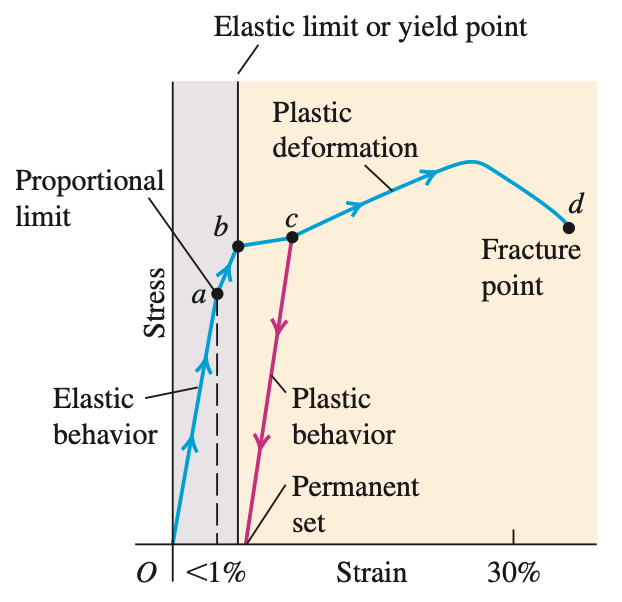
\includegraphics[scale=0.5]{stress-strain}
\end{figure}

\begin{itemize}
  \item Between points O and a Hooke's law applies and the deformation is elastic

  \item Point a is known as the proportional limit

  \item Between points a and b Hooke's law doesn't apply but the deformation is still elastic

  \item Point b is known as the yield point

  \item After point b the deformation becomes plastic

  \item At point d the material breaks

  \item Point d is known as the fracture point
\end{itemize}

\section{Fluid Mechanics}

\subsection{Gases, Liquids, and Density}

\begin{itemize}
  \item A \textbf{fluid} is any substance that can flow and change the shape of the volume it occupies — this includes gases

  \item The \textbf{density} of a material is its mass per unit volume \[\rho_\textrm{avg}=\frac{m}{V}\]

  \item The \textbf{specific gravity} of a material is the ratio of its density to the density of water at 4.0ºC
\end{itemize}

\subsection{Pressure in a Fluid}

\begin{itemize}
  \item \textbf{Pressure} is defined as \[p=\frac{F_\perp}{A}\]

  \item Pressure is measured in pascals where \[1 \textrm{ pascal}=1\textrm{ Pa}=1\textrm{ N/m}^2\]

  \item The pressure at a depth $h$ in a fluid of uniform density $\rho$ is given by \[p=p_0+\rho gh\] where $p_0$ is the pressure at the surface of the fluid

  \item \textbf{Pascal's law} states that pressure applied to an enclosed fluid is transmitted undiminished to every portion of the fluid and the walls of the containing vessel

  \item Sometimes pressure is measured relative to atmospheric pressure, e.g. a car tire, and is called \textbf{gauge pressure} otherwise it's called \textbf{absolute pressure}
\end{itemize}

\subsection{Buoyancy}

\begin{itemize}
  \item \textbf{Archimedes's Principle} states that when an object is completely or partially immersed in a fluid, the fluid exerts an upward force on the object equal to the weight of the fluid displaced by the object.
\end{itemize}

\subsection{Fluid Flow}

\begin{itemize}
  \item An \textbf{ideal fluid} is incompressible and has no internal friction (viscosity)

  \item The path of an individual particle in a moving fluid is called a \textbf{flow line}

  \item In \textbf{steady flow} the overall flow pattern doesn't change

  \item The \textbf{volume flow rate} is given by \[\frac{dV}{dt}=Av\]

  \item The \textbf{continuity equation} states that \[A_1v_1=A_2v_2\] for an incompressible fluid and \[\rho_1A_1v_1=\rho_2A_2v_2\] for a compressible fluid where $\rho$ is the density the fluid, $A$ is the cross-sectional area, and $v$ is its velocity
\end{itemize}

\subsection{Bernoulli's Equation}

\begin{itemize}
  \item \textbf{Bernoulli's equation} relates the pressure, gravitational potential energy, and kinetic energy of a fluid \[p + \rho gy + \frac{1}{2}\rho v^2 = \textrm{constant}\]

  \item Bernoulli's equation is only valid for incompressible, steady state fluid flow with no internal friction (viscosity)
\end{itemize}

\subsection{Viscosity and Turbulence}

\begin{itemize}
  \item \textbf{Viscosity} is internal friction in a fluid — the opposition of motion of one portion of fluid relative to another
\end{itemize}

\section{Gravitation}

\subsection{Newton's Law of Gravitation}

\begin{itemize}
  \item \textbf{Newton's law of gravitation} states that \[F_g=\frac{Gm_1m_2}{r^2}\] where $F_g$ is the magnitude of the attractive gravitational force between two particles, $G$ is the \textbf{gravitational constant}, $m_1$ and $m_2$ are the masses of the particles, and $r$ is the distance between them

  \item The gravitational interaction between any two spherically symmetric mass distributions is the same as if all the mass were located at their centres
\end{itemize}

\subsection{Gravitational Potential Energy}

\begin{itemize}
  \item \textbf{Gravitational potential energy} is defined as \[U=-\frac{Gm_1m_2}{r}\]
\end{itemize}

\setcounter{subsection}{3}
\subsection{The Motion of Satellites}

\begin{itemize}
  \item In a \textbf{closed orbit} the object returns to its starting point

  \item In an \textbf{open orbit} the object doesn't return to its starting point

  \item The speed of a satellite in a circular orbit around Earth is given by \[v=\sqrt{\frac{Gm_E}{r}}\]

  \item The period of a satellite in a circular orbit around Earth is given by \[T=\frac{2\pi r^{3/2}}{\sqrt{Gm_E}}\]

  \item The total energy of a satellite in a circular orbit around Earth is given by \[E=-\frac{Gm_Em}{2r}\]
\end{itemize}

\subsection{Kepler's Laws and the Motion of Planets}

\begin{itemize}
  \item \textbf{Kepler's Laws} are

        \begin{enumerate}
          \item Each planet moves in an elliptical orbit, with the sun at one focus of the ellipse

          \item A line from the sun to a given planet sweeps out equal areas in equal times

          \item The periods of the planets are proportional to the $\frac{3}{2}$ powers of the major axis lengths of their orbits
        \end{enumerate}

  \item The distance between each focus and the centre of the ellipse is $ea$ where $e$ is a dimensionless number known as the \textbf{eccentricity}

  \item If the eccentricity is 0 the two foci coincide and the ellipse is a circle

  \item The period of an object in an elliptical orbit is given by \[T = \frac {2\pi a^{3/2}}{\sqrt{GM}}\] where $a$ is the semi-major axis of the orbit and $M$ is the mass of the object that is being orbited (e.g. the sun)
\end{itemize}

\subsection{Spherical Mass Distributions}

\begin{itemize}
  \item The gravitational interaction between two spherically symmetric mass distributions is the same as though all the mass of each were concentrated at the centre

  \item Points inside a spherically symmetric mass distribution don't experience a gravitational force from mass at a greater radius from the centre
\end{itemize}

\subsection{Apparent Weight and the Earth's Rotation}

\begin{itemize}
  \item Objects that aren't at the Earth's poles undergo circular motion and must experience a net centripetal force. This force means their \textbf{apparent weight} is less than their \textbf{true weight}
\end{itemize}

\subsection{Black Holes}

\begin{itemize}
  \item The escape speed of an object with mass $M$ and radius $R$ is \[v= \sqrt \frac {2GM} R\]

  \item If the escape speed of an object is equal to $c$ it becomes a black hole

  \item If the radius of an object of mass $M$ is less than or equal to the \textbf{Schwarzchild radius} it becomes a black hole \[R_s = \frac {2GM} {c^2}\]
\end{itemize}

\section{Periodic Motion}

\subsection{Describing Oscillation}

\begin{itemize}
  \item The \textbf{amplitude} $A$ of the motion is the maximum magnitude of displacement from equilibrium

  \item A complete vibration or \textbf{cycle} is one complete round trip — from one extreme, through equilibrium, to the other extreme, through equilibrium, and back to the starting position

  \item The \textbf{period} $T$ of the motion is the duration of one cycle

  \item The \textbf{frequency} $f$ is the number of cycles per second

  \item The \textbf{angular frequency} $\omega$ is $2\pi$ times the frequency $f$

  \item Frequency and period are reciprocals of each other \[f = \frac 1 T\] \[\omega = 2\pi f = \frac {2\pi} T\]
\end{itemize}

\subsection{Simple Harmonic Motion}

\begin{itemize}
  \item When the restoring force is directly proportional to the displacement from equilibrium the oscillation is called \textbf{simple harmonic motion}

  \item An object that undergoes simple harmonic oscillation is called a \textbf{harmonic oscillator}

  \item If $k$ is the force constant of the restoring force and $m$ is the mass of the object undergoing oscillation, then \[\omega = \sqrt{\frac{k}{m}}\]

  \item This is because simple harmonic motion is analogous to uniform circular motion projected onto an axis — $\omega$ is the angular frequency of the object undergoing uniform circular motion

  \item This also means that \[f = \frac \omega {2 \pi} = \frac 1 {2\pi} \sqrt \frac k m\] and \[T = \frac 1 f = \frac {2\pi} \omega = 2 \pi \sqrt \frac m k\]

  \item The displacement of an object undergoing simple harmonic motion is \[x = A\cos(\omega t + \phi)\] where $x$ is the object's displacement, $A$ is its amplitude, $\omega$ is its angular frequency, $t$ is time, and $\phi$ is the phase angle
\end{itemize}

\subsection{Energy in Simple Harmonic Motion}

\begin{itemize}
  \item At maximum displacement from equilibrium $x=A$ and $v=0$ so \[E=K+U=\frac{1}{2}mv^2+\frac{1}{2}kx^2=\frac{1}{2}kA^2\]

  \item Only conservative forces act in simple harmonic motion, to total mechanical energy is conserved and $E=\frac{1}{2}kA^2$ always
\end{itemize}

\subsection{Applications of Simple Harmonic Motion}

\begin{itemize}
  \item Vertical SHM is the same as horizontal SHM except the equilibrium position isn't when the spring is unstretched but when its restoring force is equal to the weight of the object

  \item Under \textbf{angular SHM} \[\omega=\sqrt{\frac{\kappa}{I}}\] \[f=\frac{1}{2\pi}\sqrt{\frac{\kappa}{I}}\] \[\theta=\Theta\cos(\omega t+\phi)\] where $\Omega$ is the amplitude of the oscillation
\end{itemize}

\subsection{The Simple Pendulum}

\begin{itemize}
  \item A \textbf{simple pendulum} is an idealized model consisting of a point mass suspended by a massless, unstretchable string

  \item The restoring force for a simple pendulum is $-mg\sin\theta$ so the motion isn't SHM, however $\sin\theta \approx \theta$ for small $\theta$ in which case the motion is SHM

  \item For small $\theta$ \[k = \frac{mg}{L}\] \[\omega = \sqrt{\frac{g}{L}}\] \[f = \frac{1}{2\pi} \sqrt{\frac{g}{L}}\]
\end{itemize}

\subsection{The Physical Pendulum}

\begin{itemize}
  \item A \textbf{physical pendulum} is any real pendulum that uses an extended object, in contrast to the idealized simple pendulum with all of its mass concentrated at a point

  \item When the object is displaced from equilibrium its weight produces a restoring torque \[\tau = -mg\sin\theta\]

  \item Like the simple pendulum, this doesn't describe SHM because it's proportional to $\sin\theta$ rather than $\theta$ but it approximates SHM for small $\theta$

  \item This gives us
        \begin{align*}
          -mgd\theta           & = \tau                     \\
                               & = I\alpha                  \\
                               & = I\frac{d^2 \theta}{dt^2} \\
          -\frac{mgd}{I}\theta & = \frac{d^2 \theta}{dt^2}
        \end{align*}
        so
        \begin{align*}
          \omega & = \sqrt{\frac{mgd}{I}}      \\
          T      & = 2\pi \sqrt{\frac{I}{mgd}}
        \end{align*}
\end{itemize}

\subsection{Damped Oscillations}

\begin{itemize}
  \item The decrease in amplitude caused by dissipative forces is called \textbf{damping} and the corresponding motion is called \textbf{damped oscillation}

  \item Assuming the dissipative force on the object is proportional to its velocity such that net force is \[\Sigma F_x = -kx -bv_x\] then the displacement of a damped oscillator is described by \[x = Ae^{-(b/2m)t}\cos(\omega't + \phi)\] where \[\omega' = \sqrt{\frac{k}{m} - \frac{b^2}{4m^2}}\]

  \item When $b = 2\sqrt{km}$ then $\omega'=0$ and the condition is called \textbf{critical damping} — the system returns to its equilibrium position without oscillating

  \item When $b > 2\sqrt{km}$ then the condition is called \textbf{overdamping} — the system returns to its equilibrium position without oscillating but more slowly than under critical damping

  \item When $b < 2\sqrt{km}$ then the condition is called \textbf{underdamping} — the system oscillates with gradually decreasing amplitude

  \item The dissipative force is nonconservative so the total mechanical energy of the system decreases over time \[\frac{dE}{dt} = -bv_x^2\] which is equal to the dissipative force times velocity or the rate at which it does negative work on the system
\end{itemize}

\subsection{Forced Oscillations and Resonance}

\begin{itemize}
  \item We can maintain a constant amplitude oscillation even when damped by applying a force that varies with time in a periodic way — this force is called a \textbf{driving force}

  \item When a driving force is applied to a damped harmonic oscillator the resulting motion is called \textbf{forced oscillation}

  \item Without a driving force a system oscillates at its \textbf{natural angular frequency} $\omega'$, but with a driving force it oscillates at the driving angular frequency $\omega_d$

  \item If the driving frequency is close to the natural frequency the amplitude of oscillation increases — this is known as \textbf{resonance}

  \item The amplitude of a forced oscillator varies based on the driving frequency \[A = \frac{F_\textrm{max}}{\sqrt{(k - m\omega_d^2)^2 + b^2\omega_d^2}}\] and the amplitude is at its maximum when \[k - m\omega_d^2 = 0\] or \[\omega_d = \sqrt{\frac{k}{m}}\]
\end{itemize}

\end{document}
